\providecommand{\placeholderfigure}[3]{%
    \begin{figure}[H]
        \centering
        \fbox{%
            \parbox[c][4.0cm][c]{0.88\textwidth}{%
                \centering
                \textit{#1}%
            }%
        }
        \caption{#2}
        \label{#3}
    \end{figure}
}

\section{THIẾT KẾ KIẾN TRÚC HỆ THỐNG}
\label{sec:system-architecture-design}

Chương này trình bày kiến trúc tổng thể của hệ thống robot tự hành TurtleBot4 trong môi trường mô phỏng. Khác với Chương 2, nội dung ở đây không đi sâu lại nguyên lý của từng cảm biến mà tập trung vào cách các thành phần phần mềm và dữ liệu được tổ chức thành một hệ thống hoàn chỉnh. Mục tiêu của chương là làm rõ hệ thống gồm những package nào, mỗi package nhận dữ liệu gì, xử lý gì, xuất dữ liệu gì và phối hợp với nhau như thế nào để robot có thể tuần tra, phát hiện mục tiêu và tiếp cận mục tiêu an toàn.

\begin{figure}[H]
\centering
\resizebox{0.95\textwidth}{!}{
\begin{tikzpicture}[
  node distance=1.2cm and 1.2cm,
  block/.style={draw, rounded corners, fill=blue!5, align=center, minimum height=1cm, minimum width=2.5cm},
  >=Latex
]
\node[block, fill=gray!10] (sim) {Môi trường mô phỏng\\(Gazebo/Ignition)};
\node[block, fill=green!10, right=of sim] (sensors) {Cảm biến\\(LiDAR, RGB-D, Odom)};
\node[block, fill=orange!10, right=of sensors] (processing) {Xử lý \& Định vị\\(SLAM, YOLOv8)};
\node[block, fill=purple!10, right=of processing] (decision) {Ra quyết định\\(Mission Manager, Patrol)};
\node[block, fill=red!10, below=1.5cm of decision] (control) {Điều khiển \& Chấp hành\\(Nav2, Differential Drive)};

\draw[->, thick] (sim) -- (sensors);
\draw[->, thick] (sensors) -- (processing);
\draw[->, thick] (processing) -- (decision);
\draw[->, thick] (decision) -- (control);
\draw[->, thick] (control.west) -| (sim.south);
\end{tikzpicture}
}
\caption{Kiến trúc tổng quát của hệ thống TurtleBot4 sử dụng ROS2, SLAM, Nav2 và YOLOv8}
\label{fig:overall-system-architecture}
\end{figure}

\subsection{Tổng quan kiến trúc hệ thống}
\label{subsec:architecture-overview}

Hệ thống được thiết kế theo hướng module hóa trên ROS2. Mỗi chức năng chính được tách thành một package riêng, giao tiếp với nhau thông qua topic, action, parameter và TF. Cách tổ chức này giúp hệ thống dễ mở rộng, dễ kiểm thử và dễ thay thế từng phần mà không làm ảnh hưởng đến toàn bộ chương trình.

Về tổng thể, hệ thống có thể chia thành bốn lớp chính: lớp mô phỏng và cảm biến, lớp xử lý dữ liệu, lớp ra quyết định và lớp điều khiển chuyển động. Các lớp này tương ứng với chuỗi hoạt động từ thu nhận dữ liệu, xử lý thông tin, quyết định hành vi đến phát lệnh điều khiển cho robot.

\begin{table}[H]
    \centering
    \caption{Các lớp chức năng chính trong kiến trúc hệ thống}
    \label{tab:system-layers}
    \renewcommand{\arraystretch}{1.25}
    \small
    \begin{tabularx}{\textwidth}{|>{\raggedright\arraybackslash}p{0.22\textwidth}|>{\raggedright\arraybackslash}p{0.32\textwidth}|>{\raggedright\arraybackslash}X|}
        \hline
        \textbf{Lớp hệ thống} & \textbf{Thành phần chính} & \textbf{Vai trò trong project} \\
        \hline
        Mô phỏng và cảm biến & Gazebo/Ignition, TurtleBot4 Lite, LiDAR, camera RGB-D, odometry & Tạo môi trường thử nghiệm và sinh dữ liệu đầu vào cho hệ thống. \\
        \hline
        Xử lý dữ liệu & SLAM/localization, YOLOv8, object localization, TF & Biến dữ liệu cảm biến thành bản đồ, pose robot và pose mục tiêu. \\
        \hline
        Ra quyết định & Patrol Node, Mission Manager & Quyết định robot tiếp tục tuần tra hay chuyển sang tiếp cận mục tiêu. \\
        \hline
        Điều khiển chuyển động & Nav2, \texttt{/cmd\_vel}, differential drive & Lập kế hoạch đường đi và tạo lệnh vận tốc cho robot. \\
        \hline
    \end{tabularx}
\end{table}

Có thể mô tả tập các package chính của hệ thống như sau:

\begin{equation}
    \mathcal{P} = \left\{P_b,\, P_v,\, P_o,\, P_p,\, P_m\right\}
    \label{eq:package-set}
\end{equation}

Trong đó, $P_b$ là package bringup, $P_v$ là package vision, $P_o$ là package object localization, $P_p$ là package patrol và $P_m$ là package mission manager. Biểu thức trên nhấn mạnh hệ thống được tổ chức thành nhiều module độc lập, không phải một chương trình đơn lẻ.

\subsection{Các package chính trong hệ thống}
\label{subsec:main-packages}

\subsubsection{Package tb4\_bringup}
\label{subsubsec:tb4-bringup}

\texttt{tb4\_bringup} là package khởi chạy và cấu hình tổng thể. Package này gom các launch file, file cấu hình và công cụ hiển thị vào một điểm khởi động chung. Nó không trực tiếp nhận diện đối tượng hay điều khiển mục tiêu, nhưng có vai trò quan trọng vì bảo đảm các node được khởi động đúng thứ tự.

\begin{table}[H]
    \centering
    \caption{Vai trò của package \texttt{tb4\_bringup}}
    \label{tab:tb4-bringup}
    \renewcommand{\arraystretch}{1.25}
    \small
    \begin{tabularx}{\textwidth}{|>{\raggedright\arraybackslash}p{0.24\textwidth}|>{\raggedright\arraybackslash}X|}
        \hline
        \textbf{Mục} & \textbf{Nội dung} \\
        \hline
        Chức năng chính & Khởi chạy các node cần thiết cho toàn bộ hệ thống. \\
        \hline
        Input & Tham số launch, đường dẫn bản đồ, file cấu hình Nav2, file cấu hình SLAM, tùy chọn mở RViz. \\
        \hline
        Output & Các node được chạy đồng bộ, hệ thống sẵn sàng nhận dữ liệu cảm biến và thực hiện nhiệm vụ. \\
        \hline
        File tiêu biểu & \texttt{sim\_demo.launch.py}, \texttt{slam\_demo.launch.py}, \texttt{slam\_toolbox\_tb4.yaml}, \texttt{tb4\_debug.rviz}. \\
        \hline
        Vai trò & Giảm thao tác thủ công và bảo đảm hệ thống khởi động ổn định. \\
        \hline
    \end{tabularx}
\end{table}

\begin{figure}[H]
\centering
\begin{tikzpicture}[
  node distance=1cm and 2cm,
  block/.style={draw, rounded corners, fill=blue!5, align=center, minimum height=0.8cm},
  >=Latex
]
\node[block, fill=gray!15, minimum width=3cm] (launch) {\texttt{sim\_demo.launch.py}};
\node[block, right=of launch, yshift=2.0cm] (slam) {SLAM / Localization};
\node[block, right=of launch, yshift=1.0cm] (nav2) {Nav2};
\node[block, right=of launch, yshift=0.0cm] (vision) {YOLOv8 \& Object Loc};
\node[block, right=of launch, yshift=-1.0cm] (mission) {Mission Manager};
\node[block, right=of launch, yshift=-2.0cm] (rviz) {RViz Visualization};

\draw[->, thick] (launch.east) -- (slam.west);
\draw[->, thick] (launch.east) -- (nav2.west);
\draw[->, thick] (launch.east) -- (vision.west);
\draw[->, thick] (launch.east) -- (mission.west);
\draw[->, thick] (launch.east) -- (rviz.west);
\end{tikzpicture}
\caption{Vai trò của package \texttt{tb4\_bringup} trong quá trình khởi động hệ thống}
\label{fig:tb4-bringup-role}
\end{figure}

\subsubsection{Package tb4\_vision\_oak}
\label{subsubsec:tb4-vision-oak}

\texttt{tb4\_vision\_oak} là package nhận diện đối tượng từ ảnh RGB của camera OAK-D. Package này nhận ảnh màu, đưa ảnh vào mô hình YOLOv8n và xuất ra danh sách đối tượng được phát hiện dưới dạng detection 2D.

\begin{table}[H]
    \centering
    \caption{Input, output và vai trò của package \texttt{tb4\_vision\_oak}}
    \label{tab:tb4-vision-oak}
    \renewcommand{\arraystretch}{1.25}
    \small
    \begin{tabularx}{\textwidth}{|>{\raggedright\arraybackslash}p{0.24\textwidth}|>{\raggedright\arraybackslash}X|}
        \hline
        \textbf{Mục} & \textbf{Nội dung} \\
        \hline
        Chức năng chính & Nhận ảnh RGB, chạy YOLOv8n và publish kết quả detection 2D. \\
        \hline
        Input & Topic ảnh RGB \texttt{/oakd/rgb/preview/image\_raw}. \\
        \hline
        Output & Topic \texttt{/vision/detected\_objects}; có thể có ảnh debug \texttt{/vision/debug\_image}. \\
        \hline
        Dữ liệu xử lý & Bounding box, class id, confidence score. \\
        \hline
        Vai trò & Cung cấp thông tin ngữ nghĩa cho hệ thống, giúp robot biết mục tiêu là đối tượng nào. \\
        \hline
    \end{tabularx}
\end{table}

Một detection thứ $i$ có thể biểu diễn bởi:

\begin{equation}
    D_i = \left(u_i,\, v_i,\, w_i,\, h_i,\, c_i,\, s_i\right)
    \label{eq:detection-format}
\end{equation}

Trong đó, $(u_i, v_i)$ là tâm bounding box, $w_i$ và $h_i$ là kích thước bounding box, $c_i$ là nhãn lớp, còn $s_i$ là độ tin cậy của detection. Dữ liệu này vẫn ở dạng 2D nên cần package định vị mục tiêu để chuyển sang vị trí 3D.

\begin{figure}[H]
\centering
\begin{tikzpicture}[
  node distance=1.5cm and 2cm,
  block/.style={draw, rounded corners, fill=yellow!10, align=center, minimum height=1cm},
  >=Latex
]
\node[block, fill=blue!5] (img) {Ảnh RGB\\\texttt{image\_raw}};
\node[block] (yolo) [right=of img] {Mô hình\\YOLOv8n};
\node[block, fill=green!5] (det) [right=of yolo, align=left] {Bounding box\\Class ID\\Confidence};
\draw[->, thick] (img) -- (yolo);
\draw[->, thick] (yolo) -- (det);
\end{tikzpicture}
\caption{Luồng xử lý ảnh RGB qua YOLOv8n trong package \texttt{tb4\_vision\_oak}}
\label{fig:tb4-vision-oak-flow}
\end{figure}

\subsubsection{Package tb4\_object\_localization}
\label{subsubsec:tb4-object-localization}

\texttt{tb4\_object\_localization} là package chuyển kết quả nhận diện 2D thành vị trí mục tiêu trong không gian 3D. Package này kết hợp bounding box từ YOLOv8, ảnh depth và thông số nội tại camera.

\begin{table}[H]
    \centering
    \caption{Input, output và vai trò của package \texttt{tb4\_object\_localization}}
    \label{tab:tb4-object-localization}
    \renewcommand{\arraystretch}{1.25}
    \small
    \begin{tabularx}{\textwidth}{|>{\raggedright\arraybackslash}p{0.24\textwidth}|>{\raggedright\arraybackslash}X|}
        \hline
        \textbf{Mục} & \textbf{Nội dung} \\
        \hline
        Chức năng chính & Tính vị trí 3D của mục tiêu từ detection 2D và ảnh depth. \\
        \hline
        Input & \texttt{/vision/detected\_objects}, \texttt{/oakd/rgb/preview/depth}, \texttt{/oakd/rgb/preview/camera\_info}. \\
        \hline
        Output & \texttt{/target\_object\_pose\_map}, \texttt{/target\_object\_marker}. \\
        \hline
        Dữ liệu xử lý & Tâm bbox, giá trị depth, ma trận nội tại camera, frame cảm biến. \\
        \hline
        Vai trò & Chuyển thông tin ``thấy đối tượng trên ảnh'' thành ``mục tiêu nằm ở vị trí nào''. \\
        \hline
    \end{tabularx}
\end{table}

Nếu tâm bounding box là $(u, v)$ và độ sâu tại vùng lân cận tâm bbox là $Z$, tọa độ 3D trong hệ camera được tính theo mô hình camera lỗ kim:

\begin{equation}
    X_c = \frac{(u-c_x)Z}{f_x}, \qquad
    Y_c = \frac{(v-c_y)Z}{f_y}, \qquad
    Z_c = Z
    \label{eq:camera-to-3d}
\end{equation}

Trong đó, $f_x$, $f_y$, $c_x$ và $c_y$ được lấy từ topic camera info. Kết quả $(X_c, Y_c, Z_c)$ biểu diễn vị trí mục tiêu so với camera. Sau đó, hệ thống dùng TF để chuyển pose này sang frame phù hợp cho navigation.

\begin{figure}[H]
\centering
\begin{tikzpicture}[
  node distance=1.5cm and 2cm,
  block/.style={draw, rounded corners, fill=purple!5, align=center, minimum height=1cm},
  >=Latex
]
\node[block, fill=blue!5] (bbox) {Bounding Box\\($u, v, w, h$)};
\node[block, fill=blue!5, below=0.5cm of bbox] (depth) {Ảnh Depth\\($I_d$)};
\node[block, fill=blue!5, below=0.5cm of depth] (info) {Camera Info\\($f_x, f_y, c_x, c_y$)};
\node[block, right=of depth, minimum height=3cm] (loc) {Object\\Localization};
\node[block, fill=green!5, right=of loc] (pose) {Target Pose 3D\\($X, Y, Z$)};

\draw[->, thick] (bbox.east) -- (loc.160);
\draw[->, thick] (depth.east) -- (loc.180);
\draw[->, thick] (info.east) -- (loc.200);
\draw[->, thick] (loc.east) -- (pose.west);
\end{tikzpicture}
\caption{Quá trình chuyển bounding box và ảnh depth thành pose 3D của mục tiêu}
\label{fig:object-localization-flow}
\end{figure}

\subsubsection{Package tb4\_nav\_patrol}
\label{subsubsec:tb4-nav-patrol}

\texttt{tb4\_nav\_patrol} là package tạo hành vi tuần tra. Package này gửi lần lượt các waypoint đến Nav2 thông qua action \texttt{NavigateToPose}. Khi robot đến một waypoint, node tiếp tục gửi waypoint tiếp theo để tạo thành chu trình tuần tra.

\begin{table}[H]
    \centering
    \caption{Input, output và vai trò của package \texttt{tb4\_nav\_patrol}}
    \label{tab:tb4-nav-patrol}
    \renewcommand{\arraystretch}{1.25}
    \small
    \begin{tabularx}{\textwidth}{|>{\raggedright\arraybackslash}p{0.24\textwidth}|>{\raggedright\arraybackslash}X|}
        \hline
        \textbf{Mục} & \textbf{Nội dung} \\
        \hline
        Chức năng chính & Gửi các điểm tuần tra cho Nav2. \\
        \hline
        Input & Danh sách waypoint, trạng thái bật/tắt patrol từ Mission Manager. \\
        \hline
        Output & Goal điều hướng gửi tới action \texttt{NavigateToPose}. \\
        \hline
        Dữ liệu xử lý & Tọa độ waypoint trong frame \texttt{map}. \\
        \hline
        Vai trò & Tạo hành vi mặc định cho robot khi chưa có mục tiêu cần tiếp cận. \\
        \hline
    \end{tabularx}
\end{table}

Một waypoint có thể biểu diễn bởi:

\begin{equation}
    W_i = \left(x_i,\, y_i,\, \theta_i\right)
    \label{eq:waypoint-format}
\end{equation}

Danh sách các waypoint tuần tra được biểu diễn bởi:

\begin{equation}
    \mathcal{W} = \left\{W_1,\, W_2,\, \ldots,\, W_n\right\}
    \label{eq:waypoint-set}
\end{equation}

Trong đó, $x_i$ và $y_i$ là tọa độ waypoint trên bản đồ, còn $\theta_i$ là hướng mong muốn của robot tại điểm đó. Khi Mission Manager phát hiện mục tiêu hợp lệ, Patrol Node có thể bị tạm dừng để nhường quyền điều khiển cho nhiệm vụ tiếp cận mục tiêu.

\begin{figure}[H]
\centering
\begin{tikzpicture}[
  node distance=2.5cm,
  wp/.style={draw, circle, fill=yellow!10, align=center, minimum size=1.2cm},
  >=Latex
]
\node[wp] (w1) {$W_1$};
\node[wp, right=of w1] (w2) {$W_2$};
\node[wp, below=of w2] (w3) {$W_3$};
\node[wp, left=of w3] (w4) {$W_4$};

\draw[->, thick, dashed, bend left=15] (w1) to node[above] {Nav2} (w2);
\draw[->, thick, dashed, bend left=15] (w2) to node[right] {Nav2} (w3);
\draw[->, thick, dashed, bend left=15] (w3) to node[below] {Nav2} (w4);
\draw[->, thick, dashed, bend left=15] (w4) to node[left] {Nav2} (w1);
\end{tikzpicture}
\caption{Sơ đồ tuần tra waypoint của package \texttt{tb4\_nav\_patrol}}
\label{fig:patrol-waypoints}
\end{figure}

\subsubsection{Package tb4\_mission\_manager}
\label{subsubsec:tb4-mission-manager}

\texttt{tb4\_mission\_manager} là package điều phối hành vi cấp nhiệm vụ. Package này không xử lý ảnh trực tiếp và không điều khiển động cơ trực tiếp. Vai trò chính của nó là quyết định thời điểm robot tiếp tục tuần tra, thời điểm tạm dừng tuần tra và thời điểm gửi goal tiếp cận mục tiêu cho Nav2.

\begin{table}[H]
    \centering
    \caption{Input, output và vai trò của package \texttt{tb4\_mission\_manager}}
    \label{tab:tb4-mission-manager}
    \renewcommand{\arraystretch}{1.25}
    \small
    \begin{tabularx}{\textwidth}{|>{\raggedright\arraybackslash}p{0.24\textwidth}|>{\raggedright\arraybackslash}X|}
        \hline
        \textbf{Mục} & \textbf{Nội dung} \\
        \hline
        Chức năng chính & Điều phối giữa trạng thái tuần tra và trạng thái tiếp cận mục tiêu. \\
        \hline
        Input & Pose mục tiêu, TF giữa camera và \texttt{map}, pose robot, trạng thái Nav2. \\
        \hline
        Output & Tín hiệu bật/tắt patrol; goal tiếp cận an toàn gửi đến Nav2. \\
        \hline
        Trạng thái chính & \texttt{patrolling}, \texttt{approaching\_target}. \\
        \hline
        Vai trò & Liên kết perception với navigation ở mức hành vi. \\
        \hline
    \end{tabularx}
\end{table}

Giả sử vị trí robot và mục tiêu trong frame \texttt{map} lần lượt là:

\begin{equation}
    \mathbf{p}_r =
    \begin{bmatrix}
        x_r \\ y_r
    \end{bmatrix},
    \qquad
    \mathbf{p}_t =
    \begin{bmatrix}
        x_t \\ y_t
    \end{bmatrix}
    \label{eq:robot-target-position}
\end{equation}

Vector từ robot đến mục tiêu được tính bởi:

\begin{equation}
    \Delta \mathbf{p} = \mathbf{p}_t - \mathbf{p}_r
    =
    \begin{bmatrix}
        x_t - x_r \\
        y_t - y_r
    \end{bmatrix}
    \label{eq:robot-target-vector}
\end{equation}

Khoảng cách phẳng giữa robot và mục tiêu là:

\begin{equation}
    d = \left\lVert \Delta \mathbf{p} \right\rVert_2
    = \sqrt{(x_t-x_r)^2 + (y_t-y_r)^2}
    \label{eq:robot-target-distance}
\end{equation}

Nếu $d_s$ là khoảng cách an toàn, điểm goal tiếp cận an toàn được chọn trên đoạn thẳng từ robot đến mục tiêu:

\begin{equation}
    \mathbf{p}_g
    = \mathbf{p}_r + \frac{d-d_s}{d}\,\Delta \mathbf{p},
    \qquad d > d_s
    \label{eq:safe-goal}
\end{equation}

Khi $d \leq d_s$, robot đã đủ gần mục tiêu nên Mission Manager không cần gửi goal tiếp cận mới. Góc quay tại điểm goal có thể chọn sao cho robot hướng về mục tiêu:

\begin{equation}
    \theta_g = \operatorname{atan2}(y_t-y_g,\, x_t-x_g)
    \label{eq:safe-goal-yaw}
\end{equation}

\begin{figure}[H]
\centering
\begin{tikzpicture}[
  node distance=1.5cm and 2cm,
  block/.style={draw, rounded corners, fill=teal!5, align=center, minimum height=1cm},
  >=Latex
]
\node[block, fill=blue!5] (robot) {Robot Pose};
\node[block, fill=blue!5, below=1cm of robot] (target) {Target Pose};
\node[block, right=1.5cm of target, yshift=1cm, minimum height=2.5cm] (mm) {Mission\\Manager\\(Distance,\\Angle)};
\node[block, fill=green!5, right=of mm] (safegoal) {Safe Goal\\(Cách mục tiêu $d$)};

\draw[->, thick] (robot.east) -- (mm.150);
\draw[->, thick] (target.east) -- (mm.210);
\draw[->, thick] (mm.east) -- (safegoal.west);
\end{tikzpicture}
\caption{Sơ đồ Mission Manager tính safe goal từ pose robot và pose mục tiêu}
\label{fig:mission-manager-safe-goal}
\end{figure}

\subsection{Luồng dữ liệu chính của hệ thống}
\label{subsec:main-data-flow}

Luồng dữ liệu của hệ thống có thể chia thành ba nhánh: nhánh định vị và bản đồ, nhánh nhận diện và định vị mục tiêu, nhánh điều khiển chuyển động. Ba nhánh này gặp nhau tại Mission Manager và Nav2.

\begin{table}[H]
    \centering
    \caption{Các bước xử lý trong luồng dữ liệu chính của hệ thống}
    \label{tab:main-data-flow}
    \renewcommand{\arraystretch}{1.25}
    \small
    \begin{tabularx}{\textwidth}{|>{\centering\arraybackslash}p{0.08\textwidth}|>{\raggedright\arraybackslash}p{0.25\textwidth}|>{\raggedright\arraybackslash}X|}
        \hline
        \textbf{Bước} & \textbf{Khối xử lý} & \textbf{Dữ liệu/chức năng} \\
        \hline
        1 & Gazebo/Ignition & Sinh dữ liệu mô phỏng của robot, LiDAR, camera RGB-D và odometry. \\
        \hline
        2 & LiDAR, odometry, TF & Cung cấp dữ liệu cho SLAM/localization và Nav2. \\
        \hline
        3 & Camera RGB-D & Cung cấp ảnh RGB, ảnh depth và camera info cho nhận diện và định vị mục tiêu. \\
        \hline
        4 & YOLOv8 & Tạo detection 2D từ ảnh RGB. \\
        \hline
        5 & Object Localization & Kết hợp detection, depth và camera info để tạo pose mục tiêu. \\
        \hline
        6 & Mission Manager & Quyết định dừng patrol hay gửi goal tiếp cận mục tiêu. \\
        \hline
        7 & Nav2 & Lập kế hoạch đường đi và tạo lệnh vận tốc \texttt{/cmd\_vel}. \\
        \hline
        8 & Differential Drive & Thực thi chuyển động của robot trong môi trường. \\
        \hline
    \end{tabularx}
\end{table}

Có thể biểu diễn dữ liệu đi qua hệ thống theo chuỗi:

\begin{equation}
    I_{\mathrm{rgb}},\, I_d,\, \mathbf{K}
    \longrightarrow D_i
    \longrightarrow \mathbf{p}_{\mathrm{target}}
    \longrightarrow \mathbf{p}_{\mathrm{goal}}
    \longrightarrow \mathbf{u}
    \label{eq:main-data-chain}
\end{equation}

Trong đó, $I_{\mathrm{rgb}}$ là ảnh màu, $I_d$ là ảnh depth, $\mathbf{K}$ là ma trận nội tại camera, $D_i$ là detection, $\mathbf{p}_{\mathrm{target}}$ là pose mục tiêu, $\mathbf{p}_{\mathrm{goal}}$ là goal gửi cho Nav2 và $\mathbf{u}$ là lệnh điều khiển vận tốc.

\begin{figure}[H]
\centering
\resizebox{\textwidth}{!}{
\begin{tikzpicture}[
  node distance=1.2cm and 1.8cm,
  block/.style={draw, rounded corners, fill=orange!5, align=center, minimum height=1.2cm},
  >=Latex
]
\node[block, fill=blue!5] (cam) {Camera};
\node[block, right=of cam] (yolo) {YOLOv8\\$D_i$};
\node[block, right=of yolo] (loc) {Object Loc\\$\mathbf{p}_{\mathrm{target}}$};
\node[block, right=of loc] (mm) {Mission Mgr\\$\mathbf{p}_{\mathrm{goal}}$};
\node[block, right=of mm] (nav) {Nav2\\$\mathbf{u}$};
\node[block, fill=green!5, right=of nav] (act) {Robot Motion};

\draw[->, thick] (cam) -- node[above, font=\footnotesize] {$I_{\mathrm{rgb}}$} (yolo);
\draw[->, thick] (yolo) -- (loc);
\draw[->, thick] (loc) -- (mm);
\draw[->, thick] (mm) -- (nav);
\draw[->, thick] (nav) -- node[above, font=\scriptsize] {\texttt{/cmd\_vel}} (act);
\end{tikzpicture}
}
\caption{Luồng dữ liệu chính từ cảm biến đến lệnh điều khiển robot}
\label{fig:main-data-flow}
\end{figure}

\subsection{Sơ đồ khối kiến trúc hệ thống}
\label{subsec:system-block-diagram}

Sơ đồ khối của hệ thống nên thể hiện các module và hướng truyền dữ liệu giữa chúng. Không cần đưa quá nhiều chi tiết nội bộ của từng thuật toán trong sơ đồ này vì các nguyên lý cảm biến đã được trình bày ở Chương 2. Sơ đồ chỉ cần làm rõ package nào nhận dữ liệu nào và gửi kết quả đến đâu.

\begin{table}[H]
    \centering
    \caption{Input và output của các khối trong hệ thống TurtleBot4}
    \label{tab:system-blocks}
    \renewcommand{\arraystretch}{1.25}
    \small
    \begin{tabularx}{\textwidth}{|>{\raggedright\arraybackslash}p{0.23\textwidth}|>{\raggedright\arraybackslash}p{0.32\textwidth}|>{\raggedright\arraybackslash}X|}
        \hline
        \textbf{Khối} & \textbf{Dữ liệu vào} & \textbf{Dữ liệu ra} \\
        \hline
        Gazebo/Ignition & Mô hình robot, world warehouse & Dữ liệu cảm biến mô phỏng, \texttt{/clock}. \\
        \hline
        TurtleBot4 Sensors & Môi trường mô phỏng & \texttt{/scan}, \texttt{/odom}, RGB image, depth image, camera info. \\
        \hline
        SLAM/Localization & \texttt{/scan}, \texttt{/odom}, TF & Map, pose robot, transform \texttt{map} $\rightarrow$ \texttt{odom}. \\
        \hline
        YOLOv8 Detection & RGB image & \texttt{/vision/detected\_objects}. \\
        \hline
        Object Localization & Detection, depth, camera info & Pose mục tiêu, marker RViz. \\
        \hline
        Patrol Node & Waypoint & Goal tuần tra đến Nav2. \\
        \hline
        Mission Manager & Pose mục tiêu, pose robot, trạng thái patrol & Safe goal, tín hiệu bật/tắt patrol. \\
        \hline
        Nav2 & Map, pose robot, goal & \texttt{/cmd\_vel}. \\
        \hline
        Differential Drive & \texttt{/cmd\_vel} & Chuyển động của robot. \\
        \hline
    \end{tabularx}
\end{table}

\begin{figure}[H]
\centering
\resizebox{\textwidth}{!}{
\begin{tikzpicture}[
  node distance=1.5cm and 1.5cm,
  block/.style={draw, rounded corners, fill=gray!10, align=center, minimum height=1.2cm, minimum width=2.5cm},
  >=Latex
]
\node[block] (mission) {Mission Manager\\(Patrol / Approach)};
\node[block, left=of mission] (vision) {Vision \& Obj Loc\\(YOLOv8, Pose3D)};
\node[block, right=of mission] (nav2) {Nav2\\(Path Planning)};
\node[block, right=of nav2] (drive) {Differential Drive\\(/cmd\_vel)};

\node[block, above=1.5cm of mission] (slam) {SLAM / Loc\\(Map, TF)};
\node[block, left=of slam] (sensor) {TB4 Sensors\\(LiDAR, OAK-D)};
\node[block, left=of sensor] (sim) {Gazebo/Ignition\\(Simulation)};

\draw[->, thick] (sim) -- (sensor);
\draw[->, thick] (sensor) -- (slam);
\draw[->, thick] (sensor) -- (vision);
\draw[->, thick] (vision) -- (mission);
\draw[->, thick] (mission) -- (nav2);
\draw[->, thick] (slam) -| (nav2);
\draw[->, thick] (nav2) -- (drive);

\draw[thick] (drive.south) -- ++(0,-0.8) coordinate (tmp);
\draw[->, thick] (tmp) -| (sim.south);
\end{tikzpicture}
}
\caption{Sơ đồ khối kiến trúc module của hệ thống TurtleBot4}
\label{fig:system-module-block-diagram}
\end{figure}

\subsection{Môi trường mô phỏng}
\label{subsec:simulation-environment}

Hệ thống sử dụng Gazebo/Ignition để mô phỏng robot và môi trường warehouse. Việc mô phỏng giúp kiểm tra pipeline cảm biến, nhận diện, định vị và điều hướng trước khi triển khai lên robot thật. Trong mô phỏng, TurtleBot4 Lite được spawn vào môi trường với vị trí ban đầu đã định nghĩa.

\begin{table}[H]
    \centering
    \caption{Các thành phần trong môi trường mô phỏng}
    \label{tab:simulation-components}
    \renewcommand{\arraystretch}{1.25}
    \small
    \begin{tabularx}{\textwidth}{|>{\raggedright\arraybackslash}p{0.30\textwidth}|>{\raggedright\arraybackslash}X|}
        \hline
        \textbf{Thành phần mô phỏng} & \textbf{Vai trò} \\
        \hline
        World warehouse & Mô phỏng không gian trong nhà, hành lang, kệ hàng hoặc vật cản. \\
        \hline
        TurtleBot4 Lite & Mô hình robot di động vi sai. \\
        \hline
        LiDAR mô phỏng & Tạo dữ liệu scan dùng cho SLAM và Nav2. \\
        \hline
        Camera RGB-D mô phỏng & Tạo ảnh RGB, depth và camera info. \\
        \hline
        Odometry mô phỏng & Cung cấp ước lượng chuyển động của robot. \\
        \hline
        \texttt{/clock} & Đồng bộ thời gian mô phỏng cho các node ROS2. \\
        \hline
    \end{tabularx}
\end{table}

\begin{figure}[H]
    \centering
    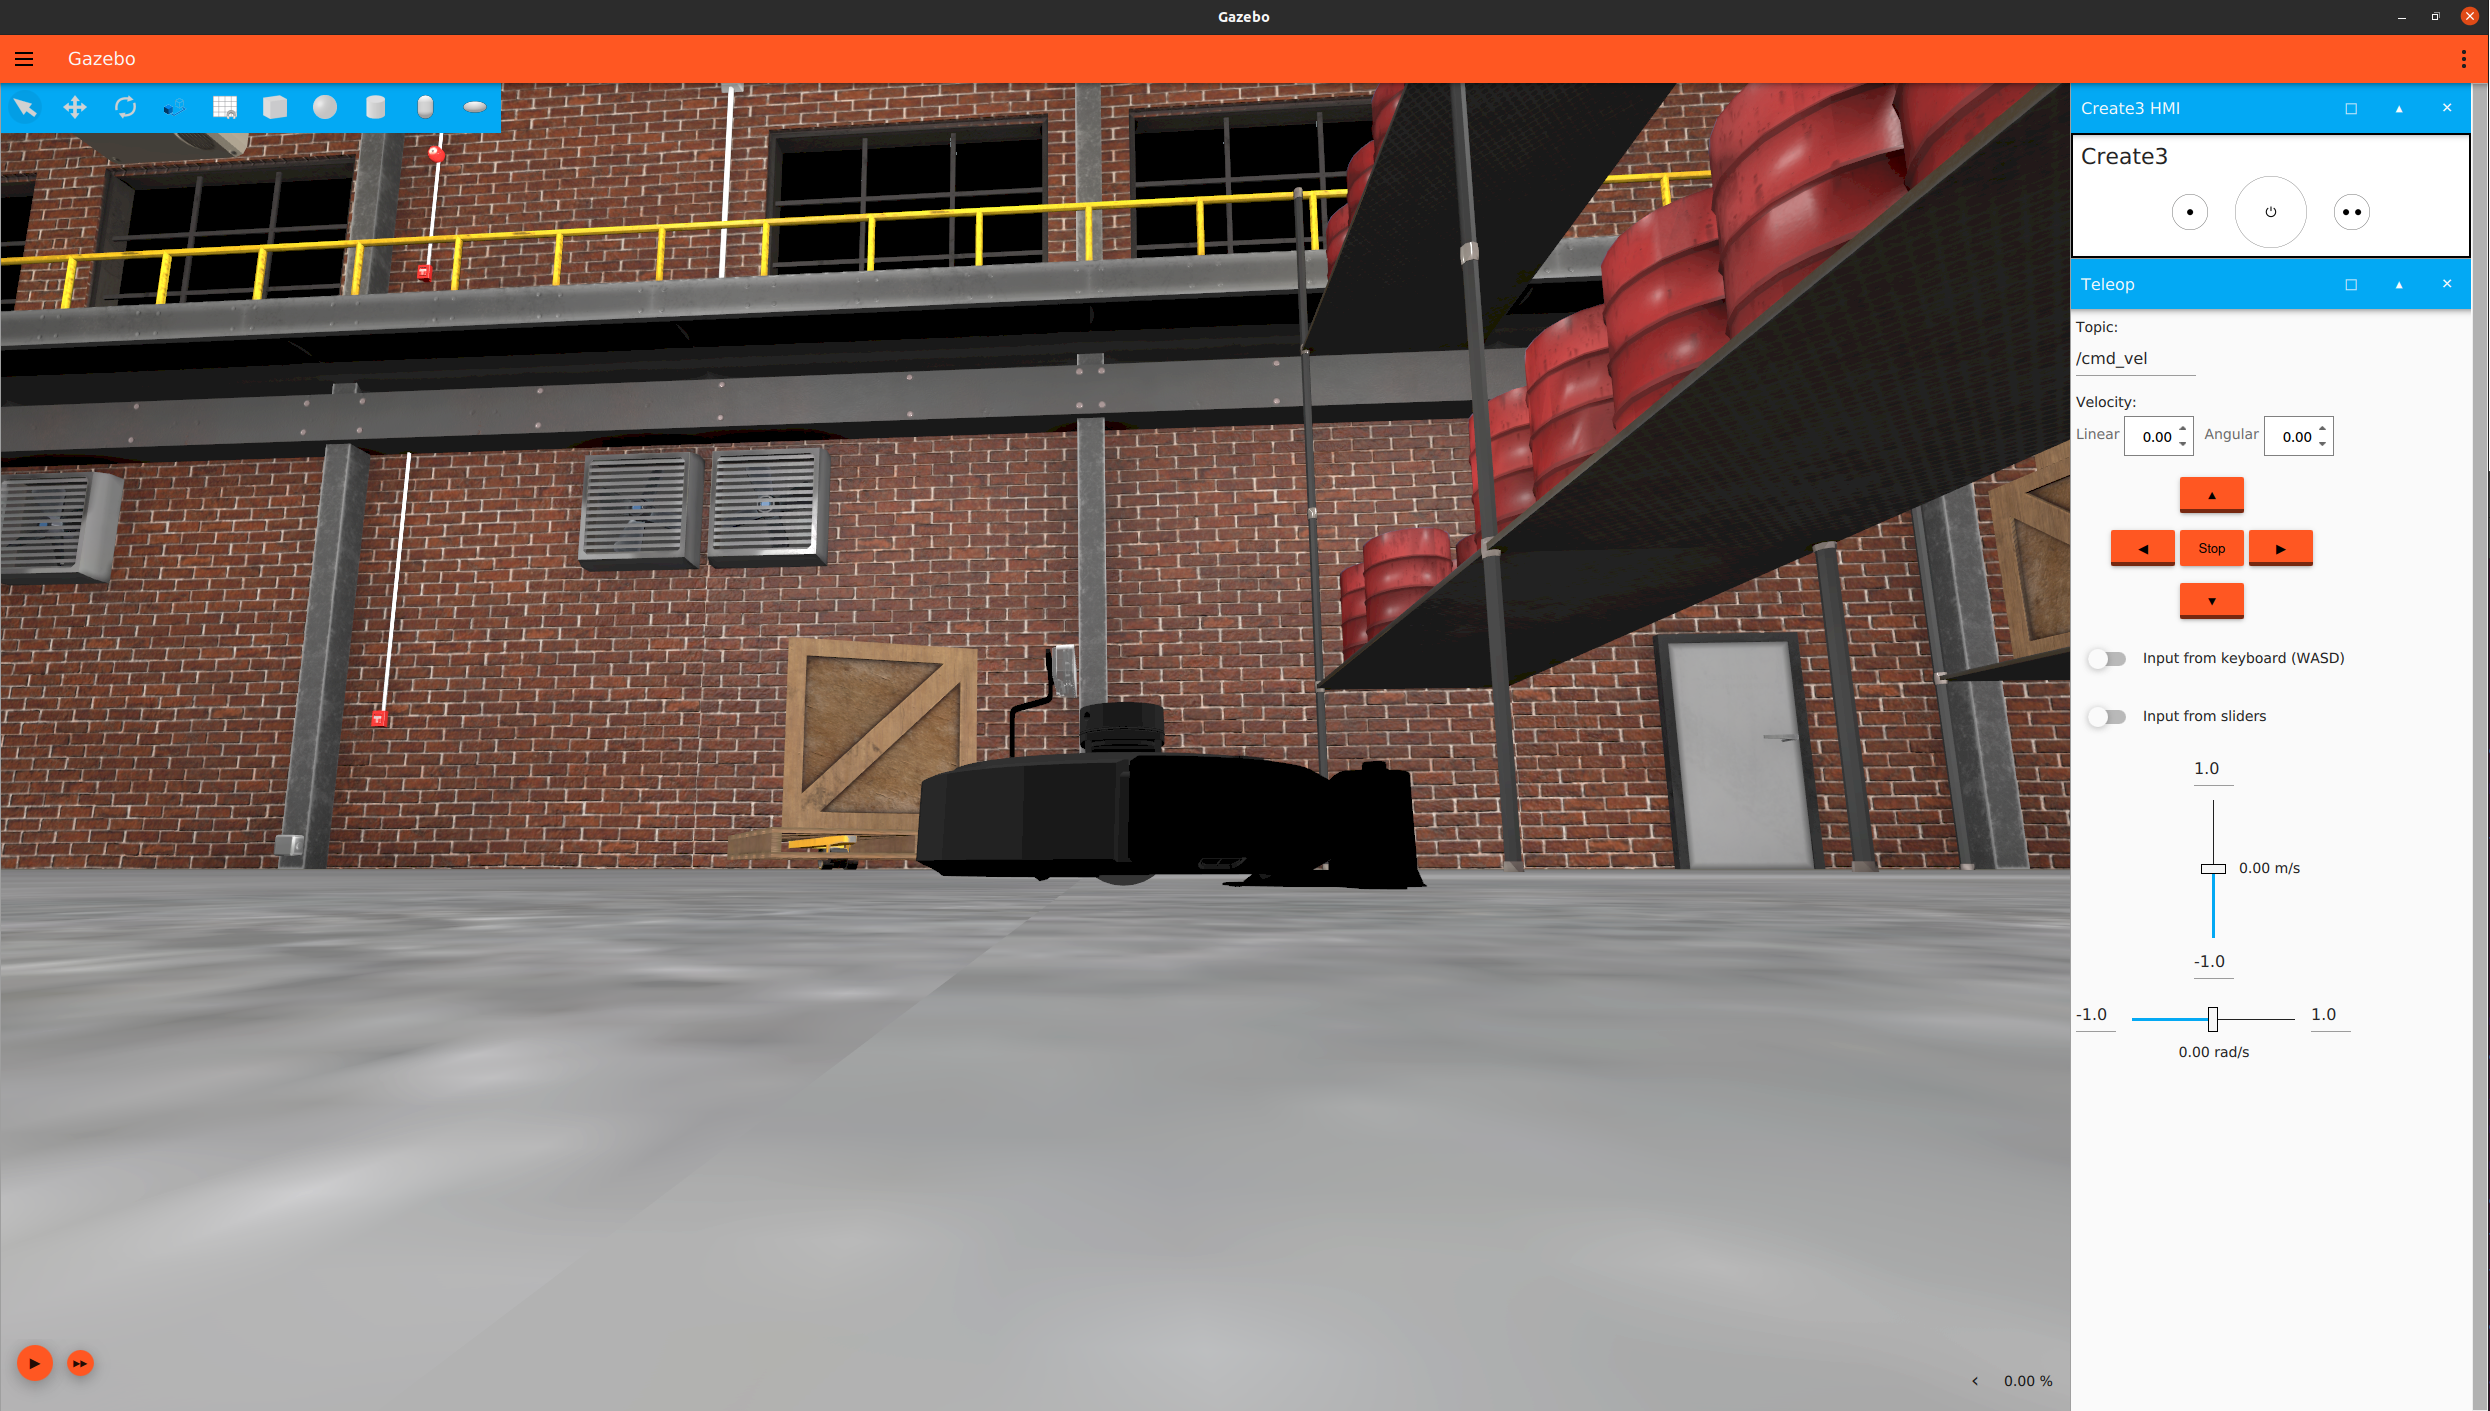
\includegraphics[width=0.85\textwidth]{images/chapter1/turtlebot4_gazebo.png}
    \caption{Môi trường mô phỏng warehouse và robot TurtleBot4 Lite trong Gazebo/Ignition}
    \label{fig:warehouse-simulation}
\end{figure}

\subsection{Cấu hình launch tổng hợp}
\label{subsec:integrated-launch-config}

Launch file tổng hợp giúp đưa toàn bộ hệ thống vào trạng thái hoạt động chỉ bằng một lệnh. Về mặt kiến trúc, đây là thành phần quan trọng vì nó giảm lỗi thao tác, thống nhất tham số và bảo đảm các node phụ thuộc nhau được khởi động hợp lý.

\begin{table}[H]
    \centering
    \caption{Các thành phần được khởi chạy bởi launch file tổng hợp}
    \label{tab:integrated-launch-components}
    \renewcommand{\arraystretch}{1.25}
    \small
    \begin{tabularx}{\textwidth}{|>{\raggedright\arraybackslash}p{0.32\textwidth}|>{\raggedright\arraybackslash}X|}
        \hline
        \textbf{Thành phần được launch} & \textbf{Mục đích} \\
        \hline
        Localization hoặc SLAM & Tạo bản đồ hoặc định vị robot trên bản đồ. \\
        \hline
        Nav2 & Nhận goal và điều hướng robot. \\
        \hline
        YOLO detection & Nhận diện mục tiêu từ ảnh RGB. \\
        \hline
        Object localization & Tính pose mục tiêu từ detection và depth. \\
        \hline
        Patrol Node & Gửi waypoint tuần tra. \\
        \hline
        Mission Manager & Điều phối hành vi tuần tra và tiếp cận. \\
        \hline
        RViz & Hiển thị map, scan, TF, marker và trạng thái robot. \\
        \hline
    \end{tabularx}
\end{table}

\begin{figure}[H]
    \centering
    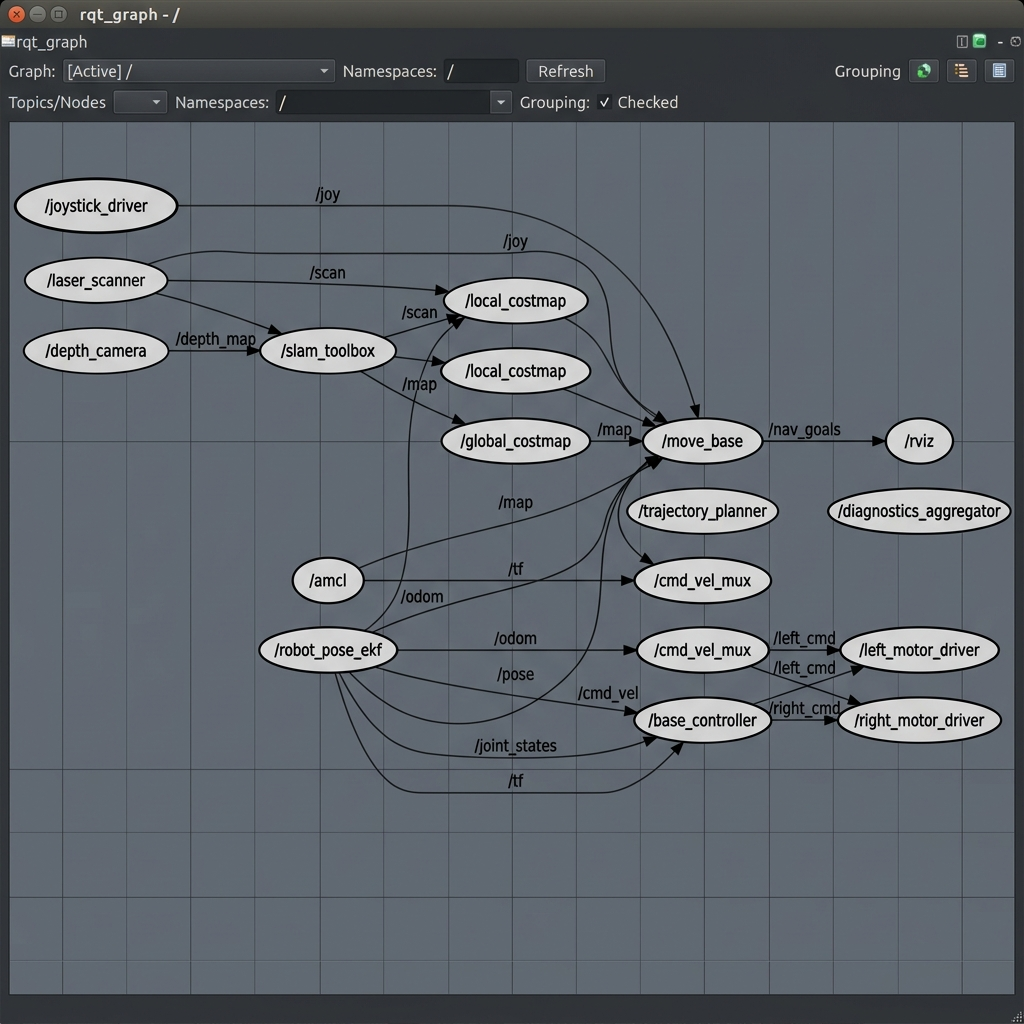
\includegraphics[width=\textwidth]{images/chapter3/rqt_graph.png}
    \caption{Quan hệ giữa launch file tổng hợp và các node được khởi chạy}
    \label{fig:integrated-launch-nodes}
\end{figure}

\subsection{Đánh giá kiến trúc hệ thống}
\label{subsec:architecture-evaluation}

Kiến trúc của hệ thống có ưu điểm là rõ ràng và dễ mở rộng. Mỗi package có một nhiệm vụ cụ thể, do đó khi cần thay đổi một chức năng, ta có thể thay package tương ứng mà không phải viết lại toàn bộ hệ thống. Ví dụ, có thể thay YOLOv8n bằng mô hình nhận diện khác mà vẫn giữ nguyên Nav2, Patrol Node và Mission Manager.

Tuy nhiên, kiến trúc này cũng phụ thuộc mạnh vào TF và đồng bộ thời gian. Nếu dữ liệu camera, depth hoặc TF không khớp thời điểm, pose mục tiêu có thể bị sai. Nếu Nav2 chưa sẵn sàng hoặc bản đồ chưa được load đúng, Mission Manager có thể gửi goal nhưng robot không di chuyển. Vì vậy, khi triển khai thực tế cần kiểm tra đầy đủ các topic, frame và trạng thái lifecycle của Nav2.

\subsection{Kết luận chương}
\label{subsec:chapter3-conclusion}

Chương này đã trình bày kiến trúc hệ thống robot tự hành TurtleBot4 theo hướng module hóa trên ROS2. Các package chính gồm \texttt{tb4\_bringup}, \texttt{tb4\_vision\_oak}, \texttt{tb4\_object\_localization}, \texttt{tb4\_nav\_patrol} và \texttt{tb4\_mission\_manager}. Mỗi package đảm nhiệm một phần trong chuỗi xử lý từ cảm biến, nhận diện, định vị mục tiêu, điều phối hành vi đến điều hướng robot. Cách thiết kế này giúp hệ thống rõ ràng, dễ kiểm thử và phù hợp với bài toán mô phỏng robot tự hành sử dụng ROS2, SLAM, Nav2 và YOLOv8.